% !TEX root = main.tex
\section{Results}
\label{sect:results}
After executing the 10-fold cross validation we can see that, Decision Tree performs better that Naive Bayes and our result matches the result in~\cite{Brunet2014a}. We achieved 94 {$\pm$} 1\% for Decision Tree and 86 {$\pm$} 1\% for the Naive Bayes classifier which matches. The accuracy of each fold of the two classifier can be visualized in Fig. \ref{fig:classification}. Also as per performance in terms of time, Naive Bayes outperformed Decision Tree by completing almost all the experiments in less than 1 second where Decision Tree took as long as almost 10 minutes in some cases.
\begin{figure}[hbt]
	\centering
	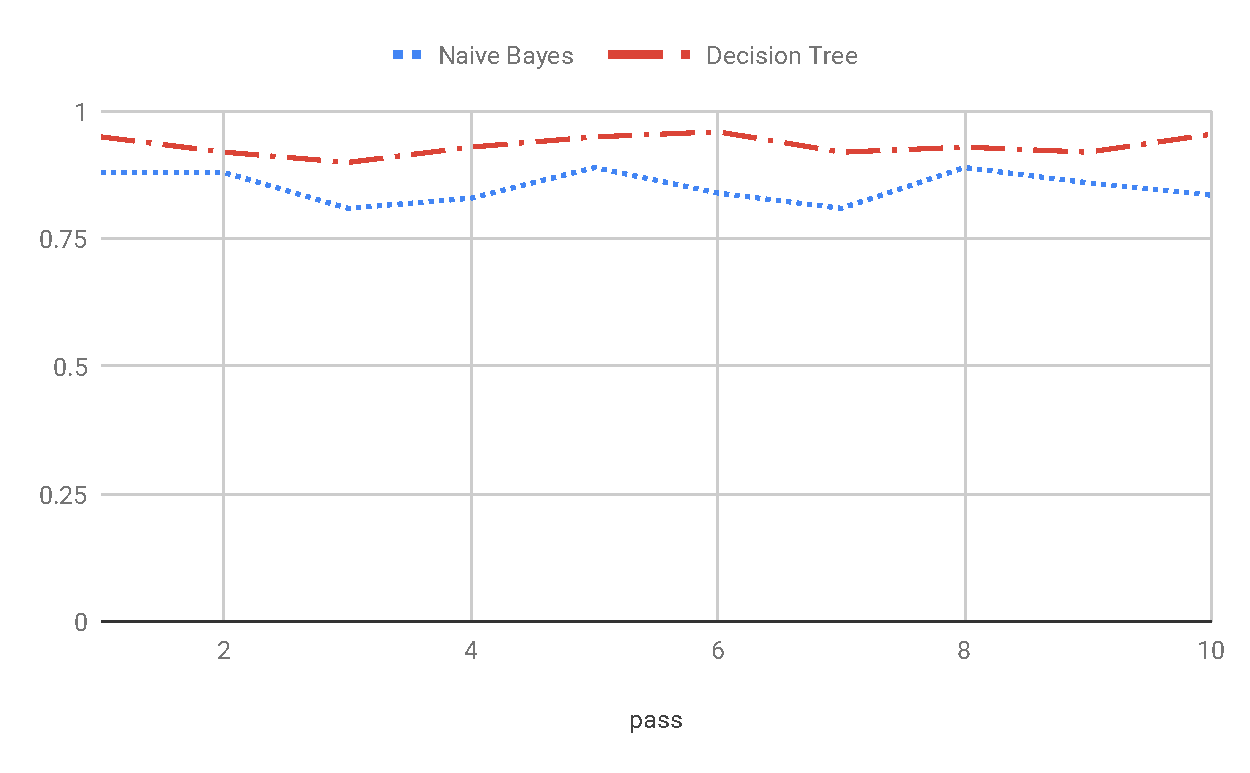
\includegraphics[width=.45\textwidth]{fig/classification.pdf}
	\caption{Accuracy of The 10-fold Validation}
	\label{fig:classification}
\end{figure}

\subsection{RQ1: To what extent do developers discuss design?}
We have used their processed data to determine the proportion of design discussions for every projects. Fig.~\ref{fig:rq_1} shows the proportion of design discussion we can see that, overall 25~{$\pm$}~6\% of the discussions in a project points to some kind of design aspect. We have also observed that our result completely matches with~\cite{Brunet2014a}.
\begin{figure}[hbt]
	\centering
	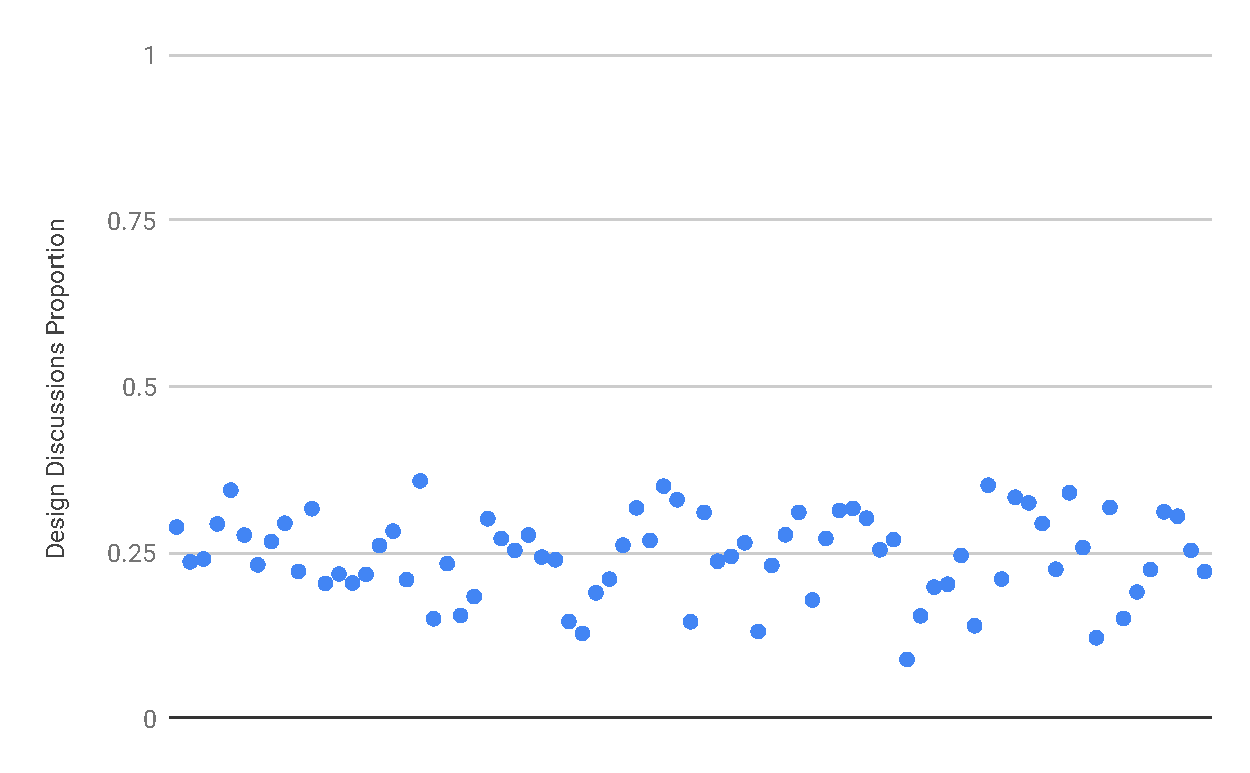
\includegraphics[width=.45\textwidth]{fig/rq_1.pdf}
	\caption{Proportion of Design Discussions Per Project}
	\label{fig:rq_1}
\end{figure}

\subsection{RQ2: Which developers discuss design?}
The authors of~\cite{Brunet2014a} analyzed data related to 22,789 developers from the 77 projects that they used. There is no information of how the developers were chosen. So we could not replicate their database pre-processing stage. So, we used their processed data to conduct the empirical study similar to them. After conducting the study, we found very similar result found by them. Similar to them, we found that the number of developers who was involved in design discussions is 8207 (36\%). Fig.~\ref{fig:rq_2}~(a) shows the proportion of contributor for each project that get involve in design discussions.
\begin{figure*}[h!]
	\subcaptionbox{Proportion of Design Discussions Contributors}{%
		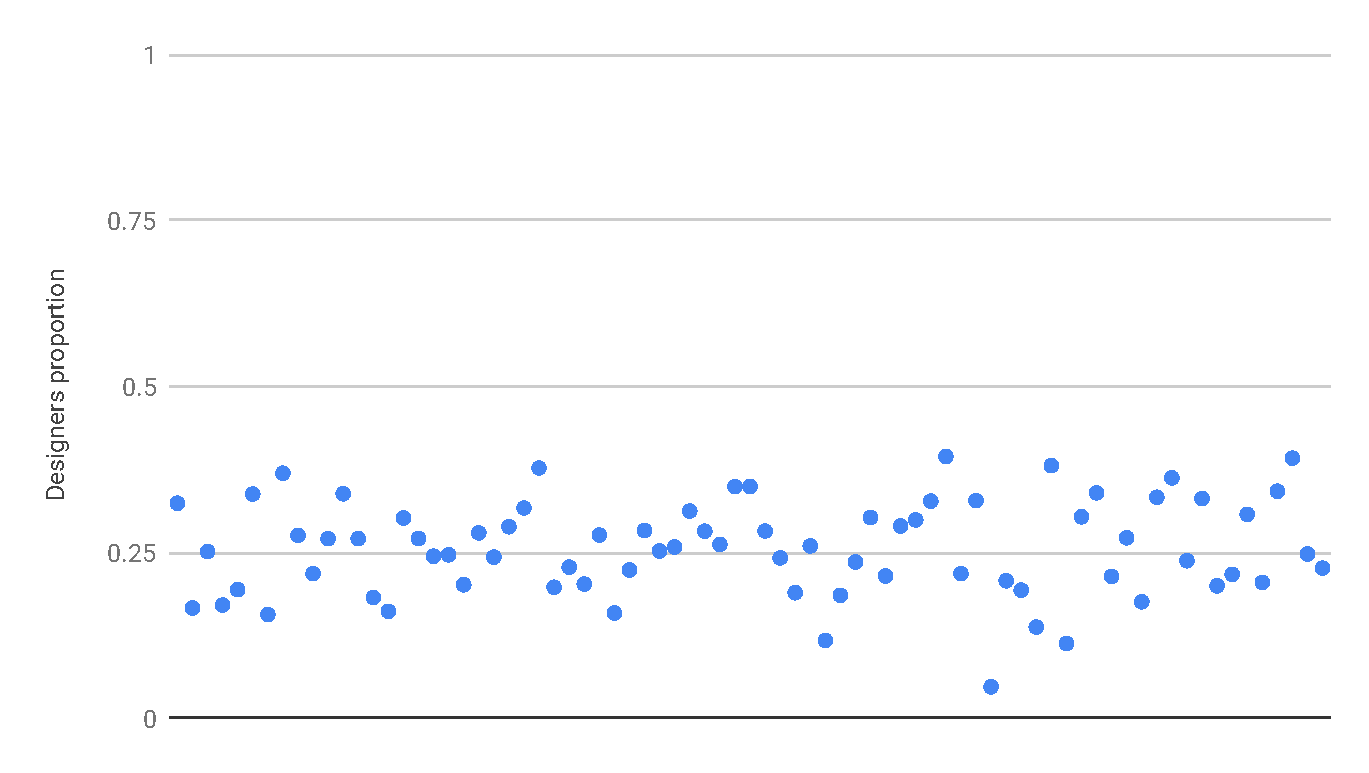
\includegraphics[width=0.30\textwidth]{fig/rq_2_a.pdf}}%
	\hfill
	\subcaptionbox{Developer's Design Discussions Coverage. X-Axis Denotes the Projects and Y-Axis Refers to the Percentage of Coverage}{%
		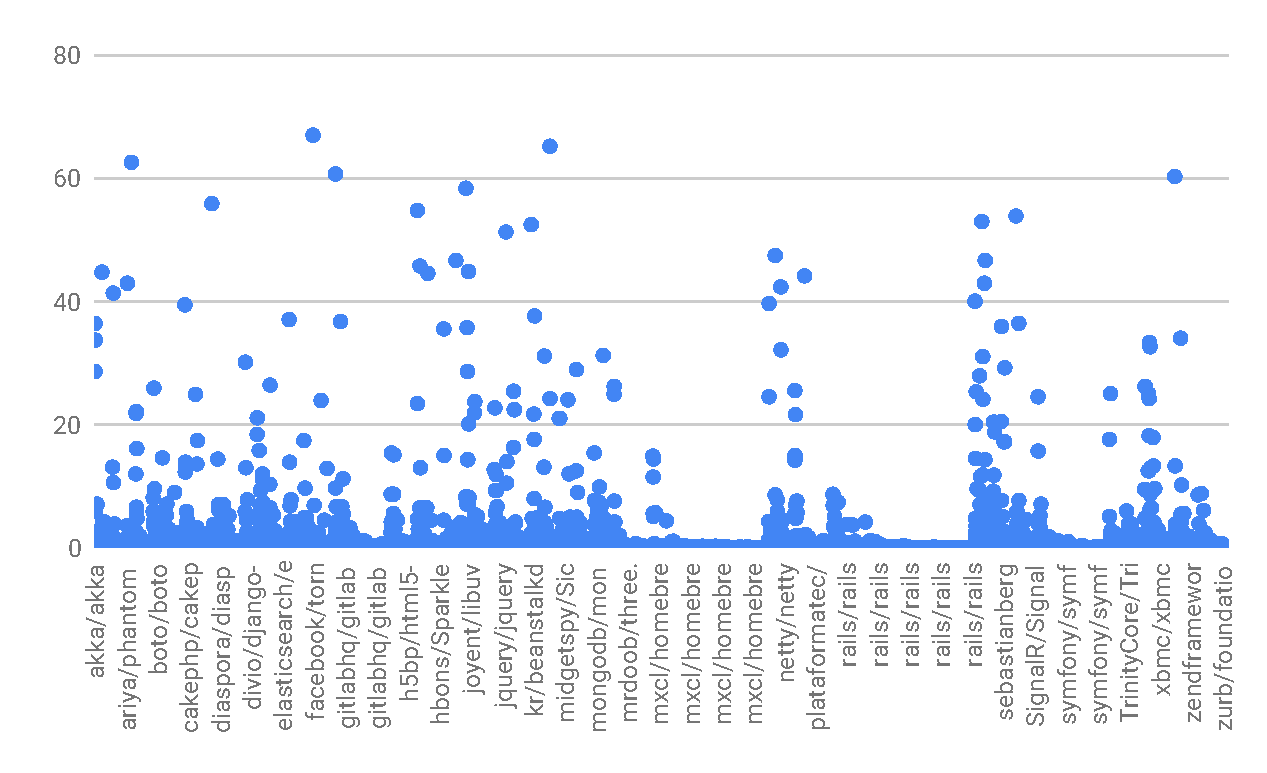
\includegraphics[width=0.30\textwidth]{fig/rq_2_b.pdf}}%
	\hfill
	\subcaptionbox{Developers Coverage with Respect to Commits}{%
		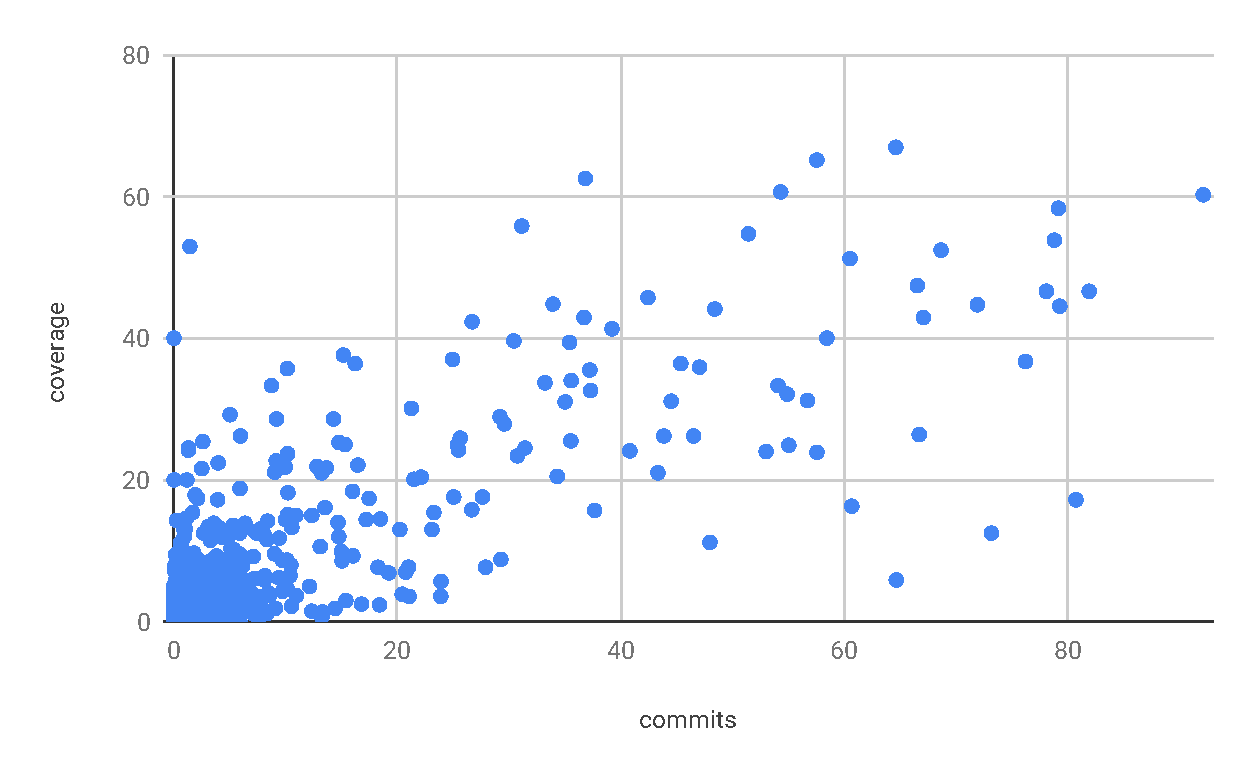
\includegraphics[width=0.30\textwidth]{fig/rq_2_c.pdf}}%
	\caption{Empirical Results}
	\label{fig:rq_2}
\end{figure*}

In the later experiments, they introduced a term called \emph{Coverage} which indicates to the proportion of all design discussions in a project to which a developer has contributed. For example, if a project has 10 design discussions and a developer contributes to 5 of them then the coverage of this developer would be 0.5. In the second step, they found that majority of developers contributes to less that 10\% of the design discussions. They also found that 99\% of the developer contribute to only 15\% of the design discussions in a specific project. After replicating this, we also have the similar conclusion. Fig.~\ref{fig:rq_2}(b) shows the coverage of developers for a specific project.

They hypothesized that several factors could be present for developers to contribute to broad range of design discussions. This scenario implies that these developers has a key role in the projects. They measured the relationship between the proportion of developers commits and their respective coverage. They used Spearman's method so did we. Eventually we found the same result as they did regarding the relation of developers commits and their coverage. Fig~\ref{fig:rq_2}(c) plots the relation between the percentage of developer commit and their coverage. We found 74\% correlation between those two parameter which is exactly the same as theirs.     
   